\documentclass[11pt]{report}
\usepackage{fancyhdr}
\usepackage{fancybox}
\usepackage{tipa}
\usepackage{framed}
\usepackage[retainorgcmds]{IEEEtrantools}
\usepackage[utf8x]{inputenc}
\usepackage{epsfig}
\usepackage[round]{natbib}
\usepackage{anysize}
\usepackage[utf8x]{inputenc}
\usepackage[english]{babel}
\usepackage{caption}
\usepackage{hyperref}
\usepackage{color,colortbl,amsmath,pifont,graphicx,amssymb}
\usepackage{url}
%\usepackage[T1]{fontenc}

%\usepackage[utf8]{inputenc}
\usepackage{floatrow}
\interfootnotelinepenalty=10000
\hypersetup{
  colorlinks   = true, %Colours links instead of ugly boxes
  urlcolor     = blue, %Colour for external hyperlinks
  linkcolor    = blue, %Colour of internal links
  citecolor   = red %Colour of citations
}

\lhead{}


\setcounter{page}{-100}
\setcounter{secnumdepth}{5}

\newenvironment{fminipage}%
{\begin{Sbox}\begin{minipage}}%
{\end{minipage}\end{Sbox}\fbox{\TheSbox}}
% Title Page
\title{\textbf{Smart-Hire}}
\vspace{2.5cm}
\author{\bf{CS620 Course Project}\\
        \\
        \\
        \emph{by}\\
        \\
        \href{http://www.cse.iitb.ac.in/~surendra/}{\bf{Surendra Salke}}\\
        \bf{Roll No : 113050003}\\
	\href{http://http://www.cse.iitb.ac.in/~bhagwatgaurav/}{\bf{Gaurav Bhagwat}}\\
        \bf{Roll No : 113050046}\\
        \\
        \emph{under the guidance of}\\
        \\
        \href{http://www.cse.iitb.ac.in/~krithi/}{\bf{Prof. Krithi Ramamrithm}}\\
	\href{http://www.cse.iitb.ac.in/~puru/}{\bf{Prof. Purushottam Kulkarni}}\\
        \\\\
        
\includegraphics[height=3.5cm]{../plots/iitb_logo}\\
        \\
        \href{http://www.cse.iitb.ac.in/}{\bf{Department of Computer Science and Engineering}}\\
        \href{http://www.iitb.ac.in/}{\bf{Indian Institute of Technology, Bombay}}\\
}
\date{May, 2013}

% page layout settings

% \setlength{\parindent}{2pc}
% \setlength{\oddsidemargin}{50pt}
% \setlength{\evensidemargin}{50pt}
% \setlength{\marginparwidth}{50pt}
% \setlength{\textheight}{9.0in}
% \setlength{\topmargin}{-0.75in}
% \setlength{\footskip}{30pt}

\marginsize{2.5cm}{2.5cm}{1cm}{1.5cm}
\setlength{\headheight}{15pt}

\pagestyle{fancy}

\begin{document}
\maketitle

\pagenumbering{roman}
\tableofcontents
\listoffigures

\begin{abstract}
In near future, electric cars can be used for daily travel. Electric cars offer energy savings and
 pollution free environment, thus can be readily deployed into public transport services. One such 
application is a case scenario where car hire services are provided by city administration and/or private 
companies.


\end{abstract}

\pagenumbering{arabic}

\chapter{Smart Hire Problem}

\section{Problem Scenario}
\begin{itemize}
\item Consider electric cars commuting all over the city. Each such battery operated car will have
its own current power level and performance­to­battery­power proportion. All of these cars are
run by the public/private company.
\item There are multiple recharging stations in the city in different areas having different recharging
costs. This is because each area in the city has different pricing policy for power at different time
of the day.
\item These charging stations are spread all over the city. The cars not currently hired can then use
those stations for charging and standby.
4. Passenger calls to the central station requesting a car at a particular time to travel from point
A to B.
\item The passenger will have some convenience index modeled on the time he/she can wait for
nearest car to come and pick him/her up.
\item The station will then respond with allotting a car which is not only the nearest possible to the
customer to reach at the requested point but also ensure that the allotted car has sufficient
power level and performance­to­power balance to complete the travel it will be hired for.
\item The stakeholder in this problem scenario is the car hire services that wants to maximize the revenue.
\end{itemize}


\section{Problem Formulation}

\subsection{Given}

\begin{itemize}
		\item The passenger’s source and destination requested and the location of all the cars with
			  respect to source. 
		\item Waiting time of each passenger. 
		\item Power levels of each car and the distance of the charging
			  stations from the passenger’s destination.
\end{itemize}


\subsection{Goals}

\begin{itemize}
	\item Maximize the service ratio.
	\item Minimize the non-revenue travel.
	\item Minimize the recharge counts.
\end{itemize}

\subsection{To Find}

\begin{itemize}
	\item Which battery (battery discharing rate) to use given the number of cars? 
	\item What number of cars achieve the goal mentioned above for a fixed
battery specification?
	\item Is there an optimal (nCars,Battery) pair for every scenario?

\end{itemize}

\subsection{Assumptions}
\begin{itemize}
	\item Cars don't recharge until they are discharged completely.
	\item Time to attend the customer apart from travel is not considered.
\end{itemize}


\subsection{Challenges}
\begin{itemize}
\item The naive method one may think is to select the car nearest from the
customer.
\item However we are limited by the amount of charge left in the car's battery
and even if the car is close to the customer's source, it may not be
able to complete the journey from source to destination.
\item Now, even if we do find a car that can fulfills the power level requirement,
it may happenthat choosing a car may render it useless for further requests as the car
may reach its depth of discharge. An unusable car would increase the waiting
time for customers even more ultimately leading to loss of revenue.


\chapter{Simulating Smart-Hire Scenario}

\section{Solution Details}

\begin{itemize}
\item The simualtion is an discrete-event simulation. Customer arrivals
are considered as 'events' and so are their departures.
\item Arrivals are registered into a global event queue according to given
arrival distribution function.
\item Customer departues events (when the car is now 'for hire') are then
automatically registered according to departure time determined by
our scheduling algorithm (as in when does customer finish its journey)
while trying to achieve our goals mentioned above.
\item The system state is captured by a 'set' of cars. With each car we track
the revenue, non-revenue, journey details. Each car has 3 states,
HIRED, FOR HIRE, UNAVAILABLE.
\item To keep a realistic scenario, we consider placing our simulation
to Mumbai city, considering only few close suburban areas (20 square miles)
example,
x cars per mile palced equally distant from each other.
\item Placement of the cars initially is ofcourse a strategic decision, however,
we dont deal with that problem and uniformly distribute the cars.
Note that the placement of cars will be same across all the simualtions.
\item We used Google Distance Matrix API for real time traffic updates and
shortest routes from source to destination.
\end{itemize}
\newpage

\section{Simulation Results: No Recharge}

\subsection{ Modeling requests }
\begin{figure}[h!t]
\centering
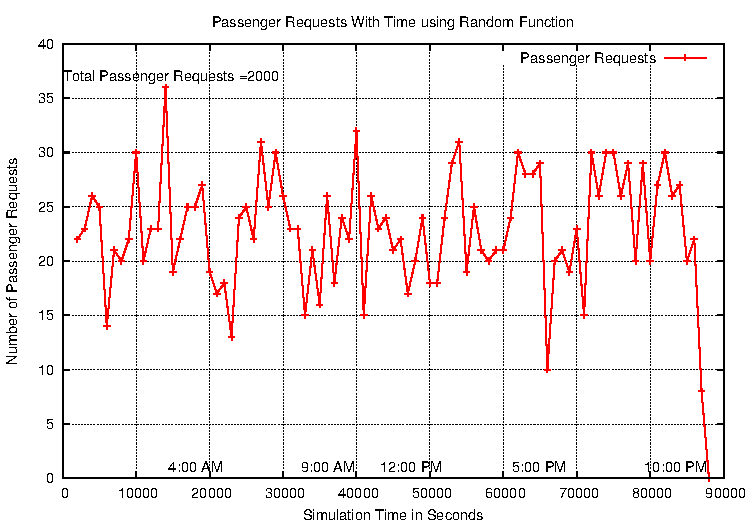
\includegraphics[scale=0.9]{../plots/passengerArrivalDistribution_old}
\caption{Passenger Arrival Requests modeled using random function}\label{fig:SVM}
\end{figure}

\begin{figure}[h!t]
\centering
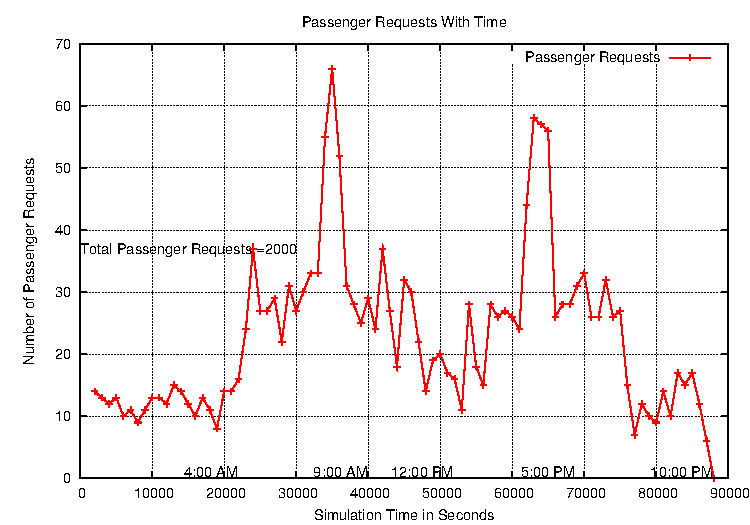
\includegraphics[scale=0.9]{../plots/passengerArrivalDistribution_9AM5PM}
\caption{Passenger Arrival Request modeled using customised function}\label{fig:SVM}
\end{figure}
\newpage

\subsection{ How does battery performance affect the service?}

\begin{figure}[h!t]
\centering
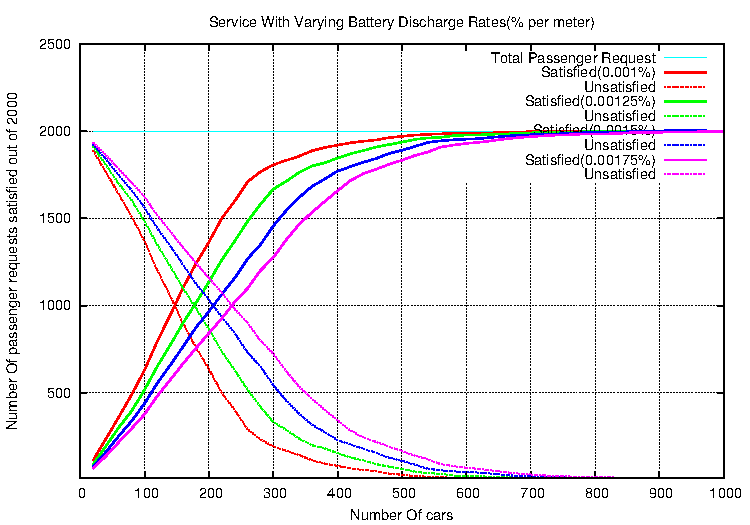
\includegraphics[scale=0.9]{../plots/nCarVariation_old}
\caption{Effect of Battery performance on service}\label{fig:SVM}
\end{figure}

\begin{itemize}
\item The expectation was that as the disharging rate increases, the service should worsen and
	  more and more cars would be rendered useless as the time progresses.
\item The service drop is expected to be linear. Less the number of cars, less is the service ratio. More the number of cars, more requests can be satisfied.	  
\item For higher battery discharing rates the results came out to be expected. However, for low discharing rates even with increasing number of cars, the requests seem to be not satisfied. 
\item The possible explanation is that even though there are large number of cars with ample battery, there are some routes that are too long to be satisfied unless some car is found with full battery.
\end{itemize}
\newpage

\subsection{ Battery behaviour }
\begin{figure}[h!t]
\centering
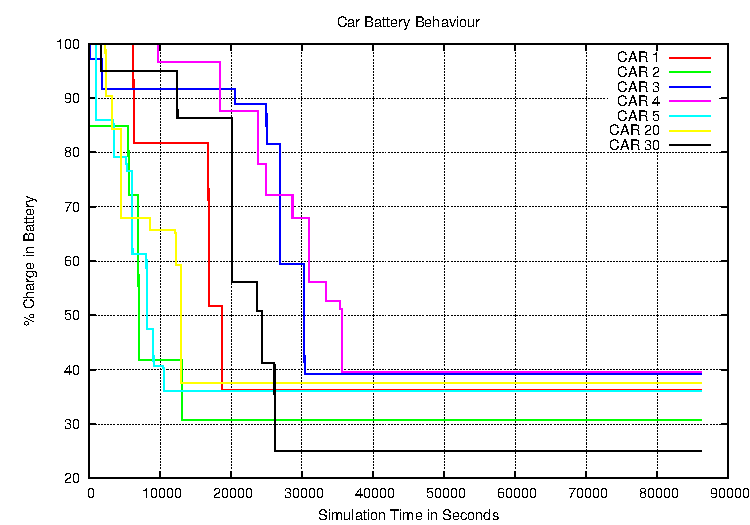
\includegraphics[scale=0.9]{../plots/carsBatteryPower}
\caption{Change in Battery charge with time}\label{fig:SVM}
\end{figure}

\subsection{ Great Losses for good guarantees of time }
\begin{figure}[h!t]
\centering
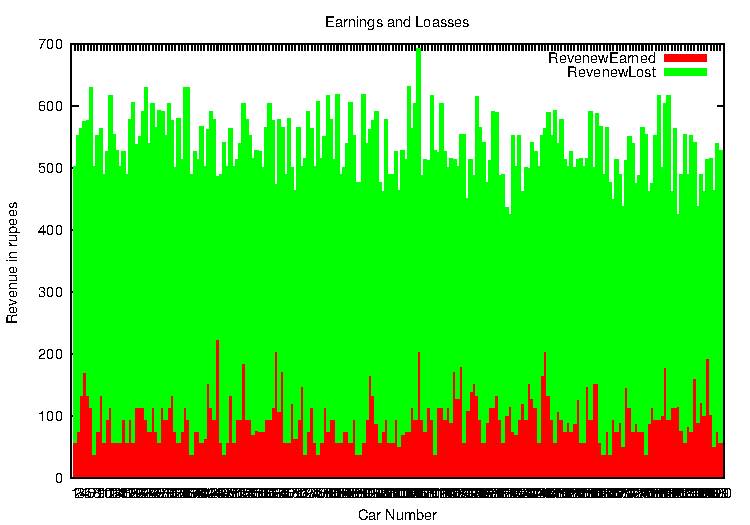
\includegraphics[scale=0.9]{../plots/EarnngsVsLosses}
\caption{Earnigs Vs Losses}\label{fig:SVM}
\end{figure}





\chapter{Conclusion}

We have only completed the scenario for no recharge so far and we have interesting results to explore this problem more. We intend to also account for
the recharging scenarios. Although one may comment that everything is heavily dependent on the customer requests, we must still expect the battery behaviour and
service to be the same.

\subsection*{Acknowledgement}
I would like to thank Prof. Krithi Ramamrithm and Prof. Purushottam Kulkarni for their constant support and guidance.% to keep me motivated.


\end{document}
